\documentclass[12pt, a4paper]{article}
\usepackage{graphicx}
\usepackage{amssymb, amsthm, amsmath}
\usepackage{indentfirst}
\usepackage{subcaption}
\usepackage{url}

\author{Elnur Gasanov}
\title{Earthquake prediction}

\parindent=0.0mm
\voffset=-40pt
\hoffset=-25pt
\textwidth=460pt

\begin{document}
\maketitle
\abstract{In this work, we address the problem of earthquake prediction using the data obtained from laboratory experiments. Initial one-dimensional feature space is transformed to many-dimensional by aggregating information about acoustic signal over many timestamps. We use Fourier and wavelet transformations (with Morlet and Mexican Hat wavelets) of the original signal along with other statistically relevant measures to obtain new features. The final model for prediction is the linear combination of XGBoost and LSTM network outputs. Usage of the latter model is reasoned by the sequential nature of the data. }

\section{Introduction}

In this paper, we try to forecast the time of the next earthquake having only some physical measurements made in the laboratory. Being able to accurately predict when an earthquake will happen may help to diminish repercussions of the disaster.

Recent advances in machine learning can be used for solving the problem stated. In \cite{MachineLearningPredicts}, random forests are used to predict time until the next earthquake, whereas in \cite{XGBoostPaper} XGBoost is applied to tackle the same problem. Both models aggregate data derived from multiple time instances of the original physical signal using approximately 100 statistical features and predict time until the next failure for the specific window using only those features. 

We substantially increase the number of features using wavelet transformations \cite{wavelet}. Wavelet transforms are well-known for describing the original signal in frequency-spatial domain. The magnitudes of signals constituting the original time series might be helpful in increasing overall accuracy of the model.

In our model we use Recurrent Neural Networks, which are universally acknowledged as the powerful tool in such tasks as language modelling, handwriting recognition and generation, machine translation, speech recognition. RNNs work well \cite{karpathy} when the data has sequential nature. We make use of RNNs to capture sequential patterns which are inherent in our dataset.

All the data is taken from Kaggle competition "LANL Earthquake Prediction" \cite{Competition}.

\section{Signal transformation}

 In the beginning, we replace all values of the acoustic signal which do not lie the frame [mean - 3 std, mean + 3 std] by the extreme values of the frame. Then, we divide the original acoustic signal to segments of the same window size $w_s$. For each time window, we compute around 200 statistical features (mean, standard deviation, quantile, sta/lta, etc.) (see \cite{Kernel}). In addition to this, we calculate mean, standard deviation, maximum and minimum values for scalograms derived from the signal. Unlike the Fourier transformation, wavelet transformation \cite{wavelet} can determine the magnitude of a signal in the spatial frequency domain. The following formula defines the wavelet transform:
$$
[W_{\psi} \phi] (a, t') = \frac{1}{|a|} \sum_t \psi\left(\frac{t - t'}{a}\right) \phi(t),
$$
where $a$ denotes scale, which controls the frequency we observe, $t'$ ranges over all time stamps of the signal, $\psi$ is a wavelet. 
We use Morlet and Mexican Hat wavelets. Information from the transformed signal, later on, is aggregated over a window of size 5000. Total number of features is approximately $200 + 16 \frac{w_s}{5000}$. 

\section{Training models}

Both models (XGBoost \cite{xgboost} and recurrent neural network \cite{lstm}) are trained independently from each other. We used a grid search with 5-fold cross-validation to find the best hypermeters for XGBoost. For the boosting algorithm $w_s = 15 \cdot 10^4$. Since test data for the competition \cite{Competition} consists of signals of length $15 \cdot 10^4$, for training RNN we divided the original signal into frames of size $3 \cdot 10^4$, so that RNN's response is obtained based on five objects. Feature matrix size for RNN has shapes (20971, 465). It turned out to be that a 2-layered LSTM network with hidden dimension 64 predicted labels much better than a 1-layered network. To speed up the learning process we add a normalization layer after two LSTM layers. RNN tended to overfit the train data, which is 80\% of all the data available. To avoid this dropout layers with dropout probability 0.7 and regularization were added to the final RNN model.  Loss minimized during backpropagation process had the following form:

$$
\text{Loss} = \frac{1}{|{\text{Train}}|} \sum\limits_i (net(x_i) - y_i)^2 + 5 \cdot 10^{-5} (\| w \|_1 + \| w \|_2).
$$

Adam with stepsize $5 \cdot 10^{-3}$ was launched to minimize the loss.

The output of the combined model is the average of XGBoost and RNN outputs.

\section{Results}

Results of testing models are presented in table~\ref{tab}. As can be seen from it, the combined model shows better performance than each model separately. However, 
there are glaringly obvious markers of uncertain prediction of each model in figures~\ref{pic1} and~\ref{pic2}. The best model of the competition gives a mean absolute error of 1.28 on 13\% of the test data with unavailable labels while our model gives the score of 1.548.

\begin{table}
\centering
\begin{tabular}{|c|c|}
\hline
Method & Mean absolute error \\
\hline
Baseline approach & 3.25 \\
\hline
RNN & 2.43 \\
\hline
XGBoost & 2.53 \\
\hline
Combined model & 2.38 \\
\hline
\end{tabular}
\caption{Results of experiments. Test data is last 20\% of all the data available for supervised learning. Baseline approach predicts all labels by one number, which is the average of all labels in the test data. The combined model shows better performance on hold-out data.}
\label{tab}
\end{table}

\begin{figure*}[t!]
    \centering
    \begin{subfigure}[t]{0.5\textwidth}
        \centering
        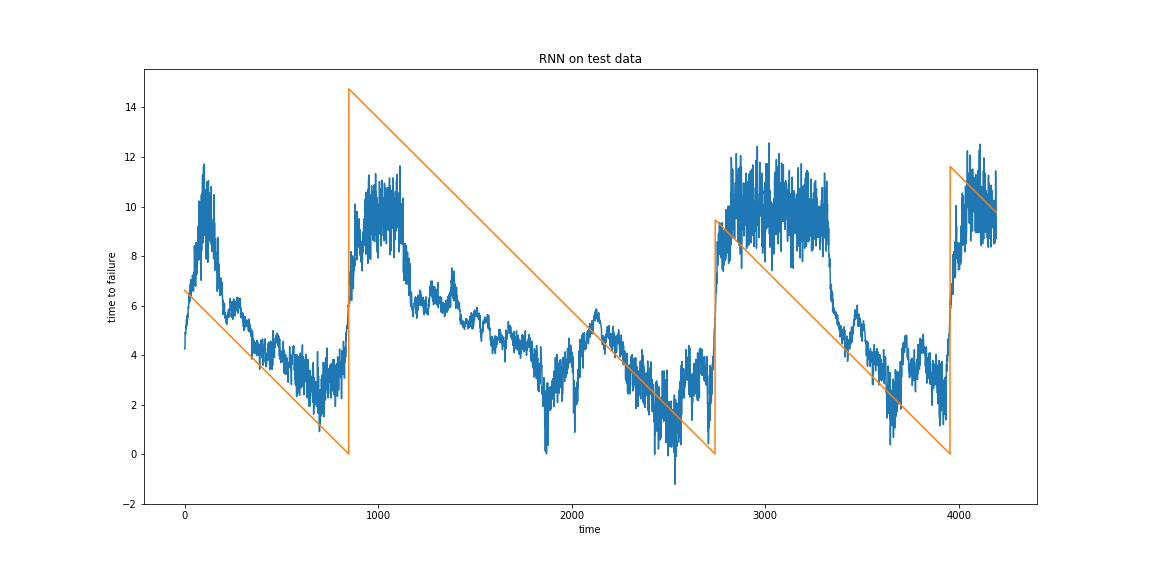
\includegraphics[width=\linewidth]{RNN_on_test_data.png}
        \caption{RNN results on the test data}
        \label{pic1}
    \end{subfigure}%
    ~ 
    \begin{subfigure}[t]{0.5\textwidth}
        \centering
        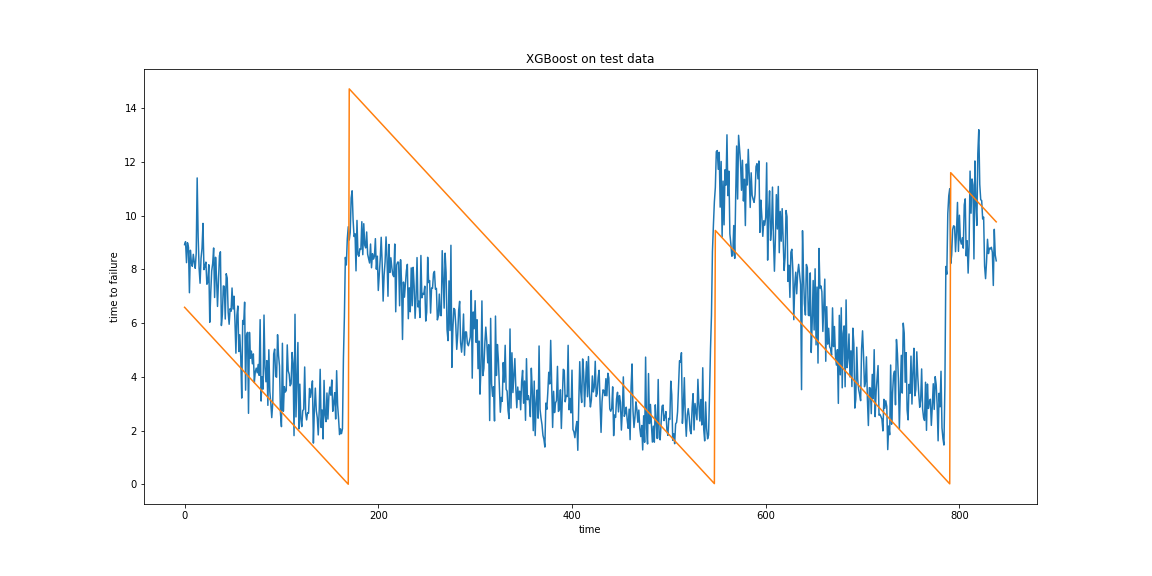
\includegraphics[width=\linewidth]{xgboost_on_test_data.png}
        \caption{XGBoost results on the test data}
        \label{pic2}
    \end{subfigure}
    \caption{Outputs of each model on the test data, which is last 20\% of all the data. Orange curve shows the real labels (time till the next failure), blue curve is the output of the models. RNN often highly either underestimates or overestimates time till the failure.}
\end{figure*}

\section{Future work and conclusion}

Both models show high uncertainty. The better approach to tackle the problem may lie in combining a higher number of models in order to decrease overall uncertainty. Moreover, instead of averaging outputs, one can apply a convex combination, which can differ depending on the data point: it means that feature space is divided into areas and different models give a different level of certainty about their outputs depending on the area. 

\bibliographystyle{plain}
\bibliography{reference.bib}



\end{document}